\section{Landscape of particle dark matter theory}
\label{sec:theory}

%\subsection{Landscape of theories proposing particle dark matter}
%10,000 foot overview of theories that predict dark matter particles in this mass range. Note any interesting properties of the predicted particles, e.g., requires spin-dependent or EFT coupling, Can we say something about their preferred cross-section ranges in a finite number of plots?



The scope of particle dark matter models has evolved since the 1970's when the necessity for Beyond Standard Model (BSM) physics to account for the dark matter in the Universe became evident, resulting in a plethora of diverse ideas today. In the 1980's, BSM models were largely motivated by solving other problems of the Standard Model (SM), containing dark matter candidates almost as an afterthought. This is, for example, the case of supersymmetric versions of the SM (SSM), of which many non-minimal variations (NMSSM) are at the moment compatible with existing experimental limits. In the 1990's, the inclusion of good dark matter candidates became essentially mandatory for all proposed BSM models. At that time, most of the attention focused on the case where the dark matter interactions are feeble due to the exchange of heavy mediators. Since the 2000's and onward, a paradigm shift occurred in which many dark matter models are proposed to fit hints from experiments and/or predict novel dark matter signatures and experiments, with less attention to their completeness, although many nonetheless have implications at accelerators, e.g. searching for light mediators and/or displaced vertices. This has blossomed into exploring many types of dark interactions, and even whole “dark sectors” connected to the SM through “portals” leading to very small couplings with photons, neutrinos, or the Higgs boson. 

 Many of these models predict scattering cross sections with nuclei and/or electrons close to the neutrino fog in multi-ton direct detection experiments, although the magnitude of the cross section often spans a wide range. In the following, we classify models in terms of this feature as schematically shown in Fig.~\ref{fig:lanscape_theory} and mention a few of each type which predict scattering cross sections close to the neutrino fog. We restrict our discussion to only examples in which regions of the scattering cross section versus mass are presented by the authors, some of which we reproduce in our figures. Overviews of these models can be found e.g. in \cite{Battaglieri:2017aum}  or \cite{Billard:2021uyg}. 
 
 The relevance of the neutrino background depends on the  dark matter scattering spectrum. The neutrino fog for dark matter scattering off nuclei we mention in this section refers to Spin Independent (SI) interaction and we reproduce in the figures its level for xenon~\cite{Billard:2013qya,Ruppin:2014bra}.  The effect of the neutrino background is much less pronounced for other types of interactions with momentum suppressed elastic  scattering cross sections and for inelastic scattering (see e.g.~\cite{Gelmini:2018ogy}). The spectrum of dark matter scattering off electrons is always different from the neutrino background spectrum. However this background still has an impact in the discovery reach that depends on the exposure~\cite{Essig:2018tss,Wyenberg:2018eyv}.  
 \begin{figure}[t]
\begin{center}
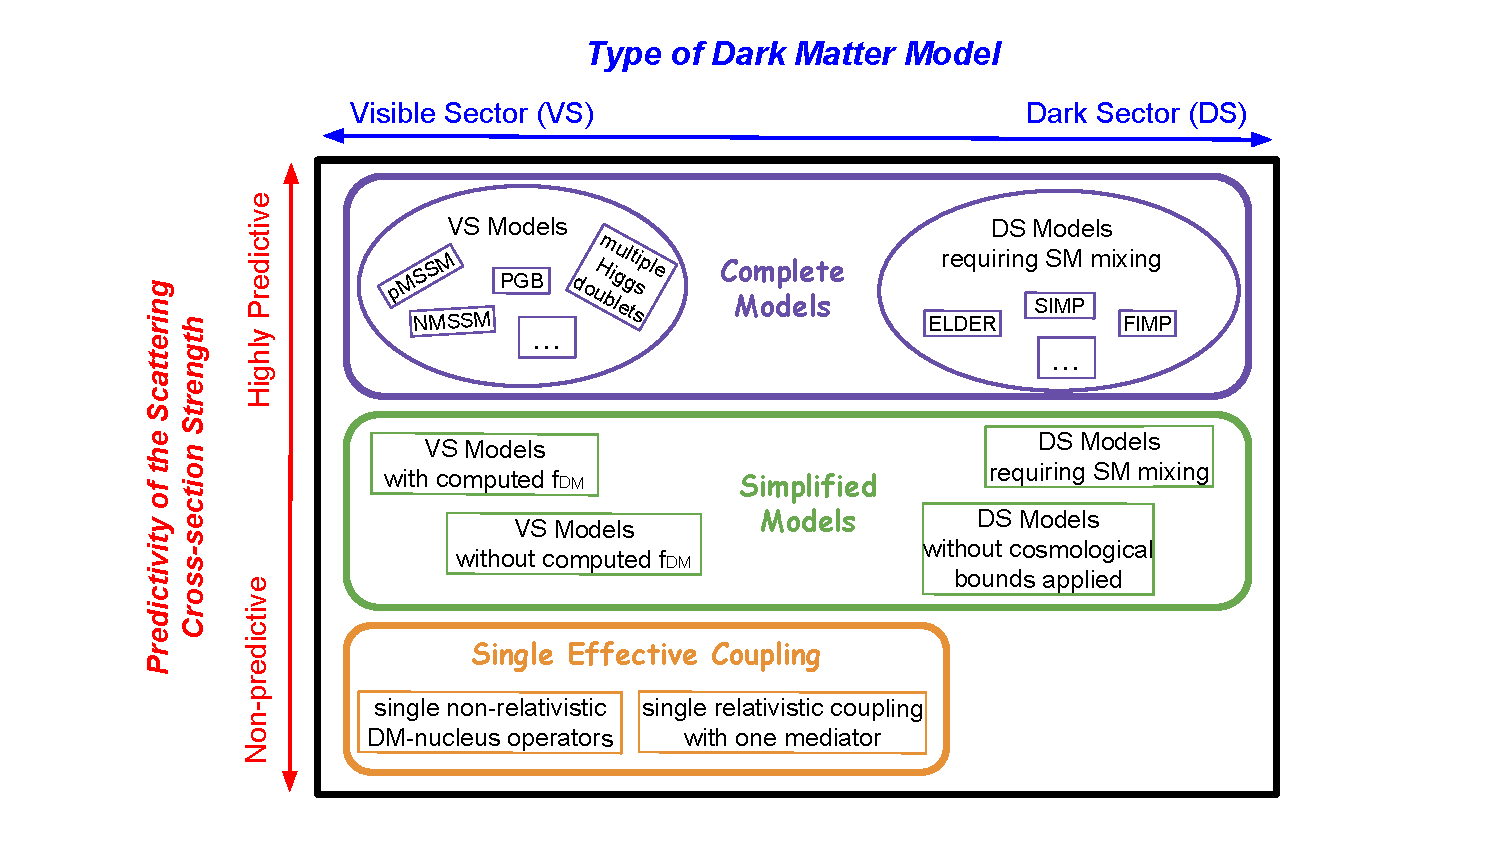
\includegraphics[width=1.0\columnwidth]{figures/model_classification.pdf}
\caption{Landscape of models classified in terms of predictivity of scattering cross sections strength with nuclei or electrons (vertical axis) and from mostly built within the visible sector or a dark sector (horizontal axis), as explained in the text.  Complete models are highly predictive, single effective coupling models are non-predictive, and simplified models are somewhere in between, in terms of predictivity. Examples of models that predict cross sections at the neutrino fog level are given in the text (FIMP or feebly interacting massive particles models typically predict  cross sections much below the neutrino fog level in the dark matter mass range of interest here).  
}
\label{fig:lanscape_theory}
\end{center}
\end{figure}

\begin{figure}[t]
\begin{center}
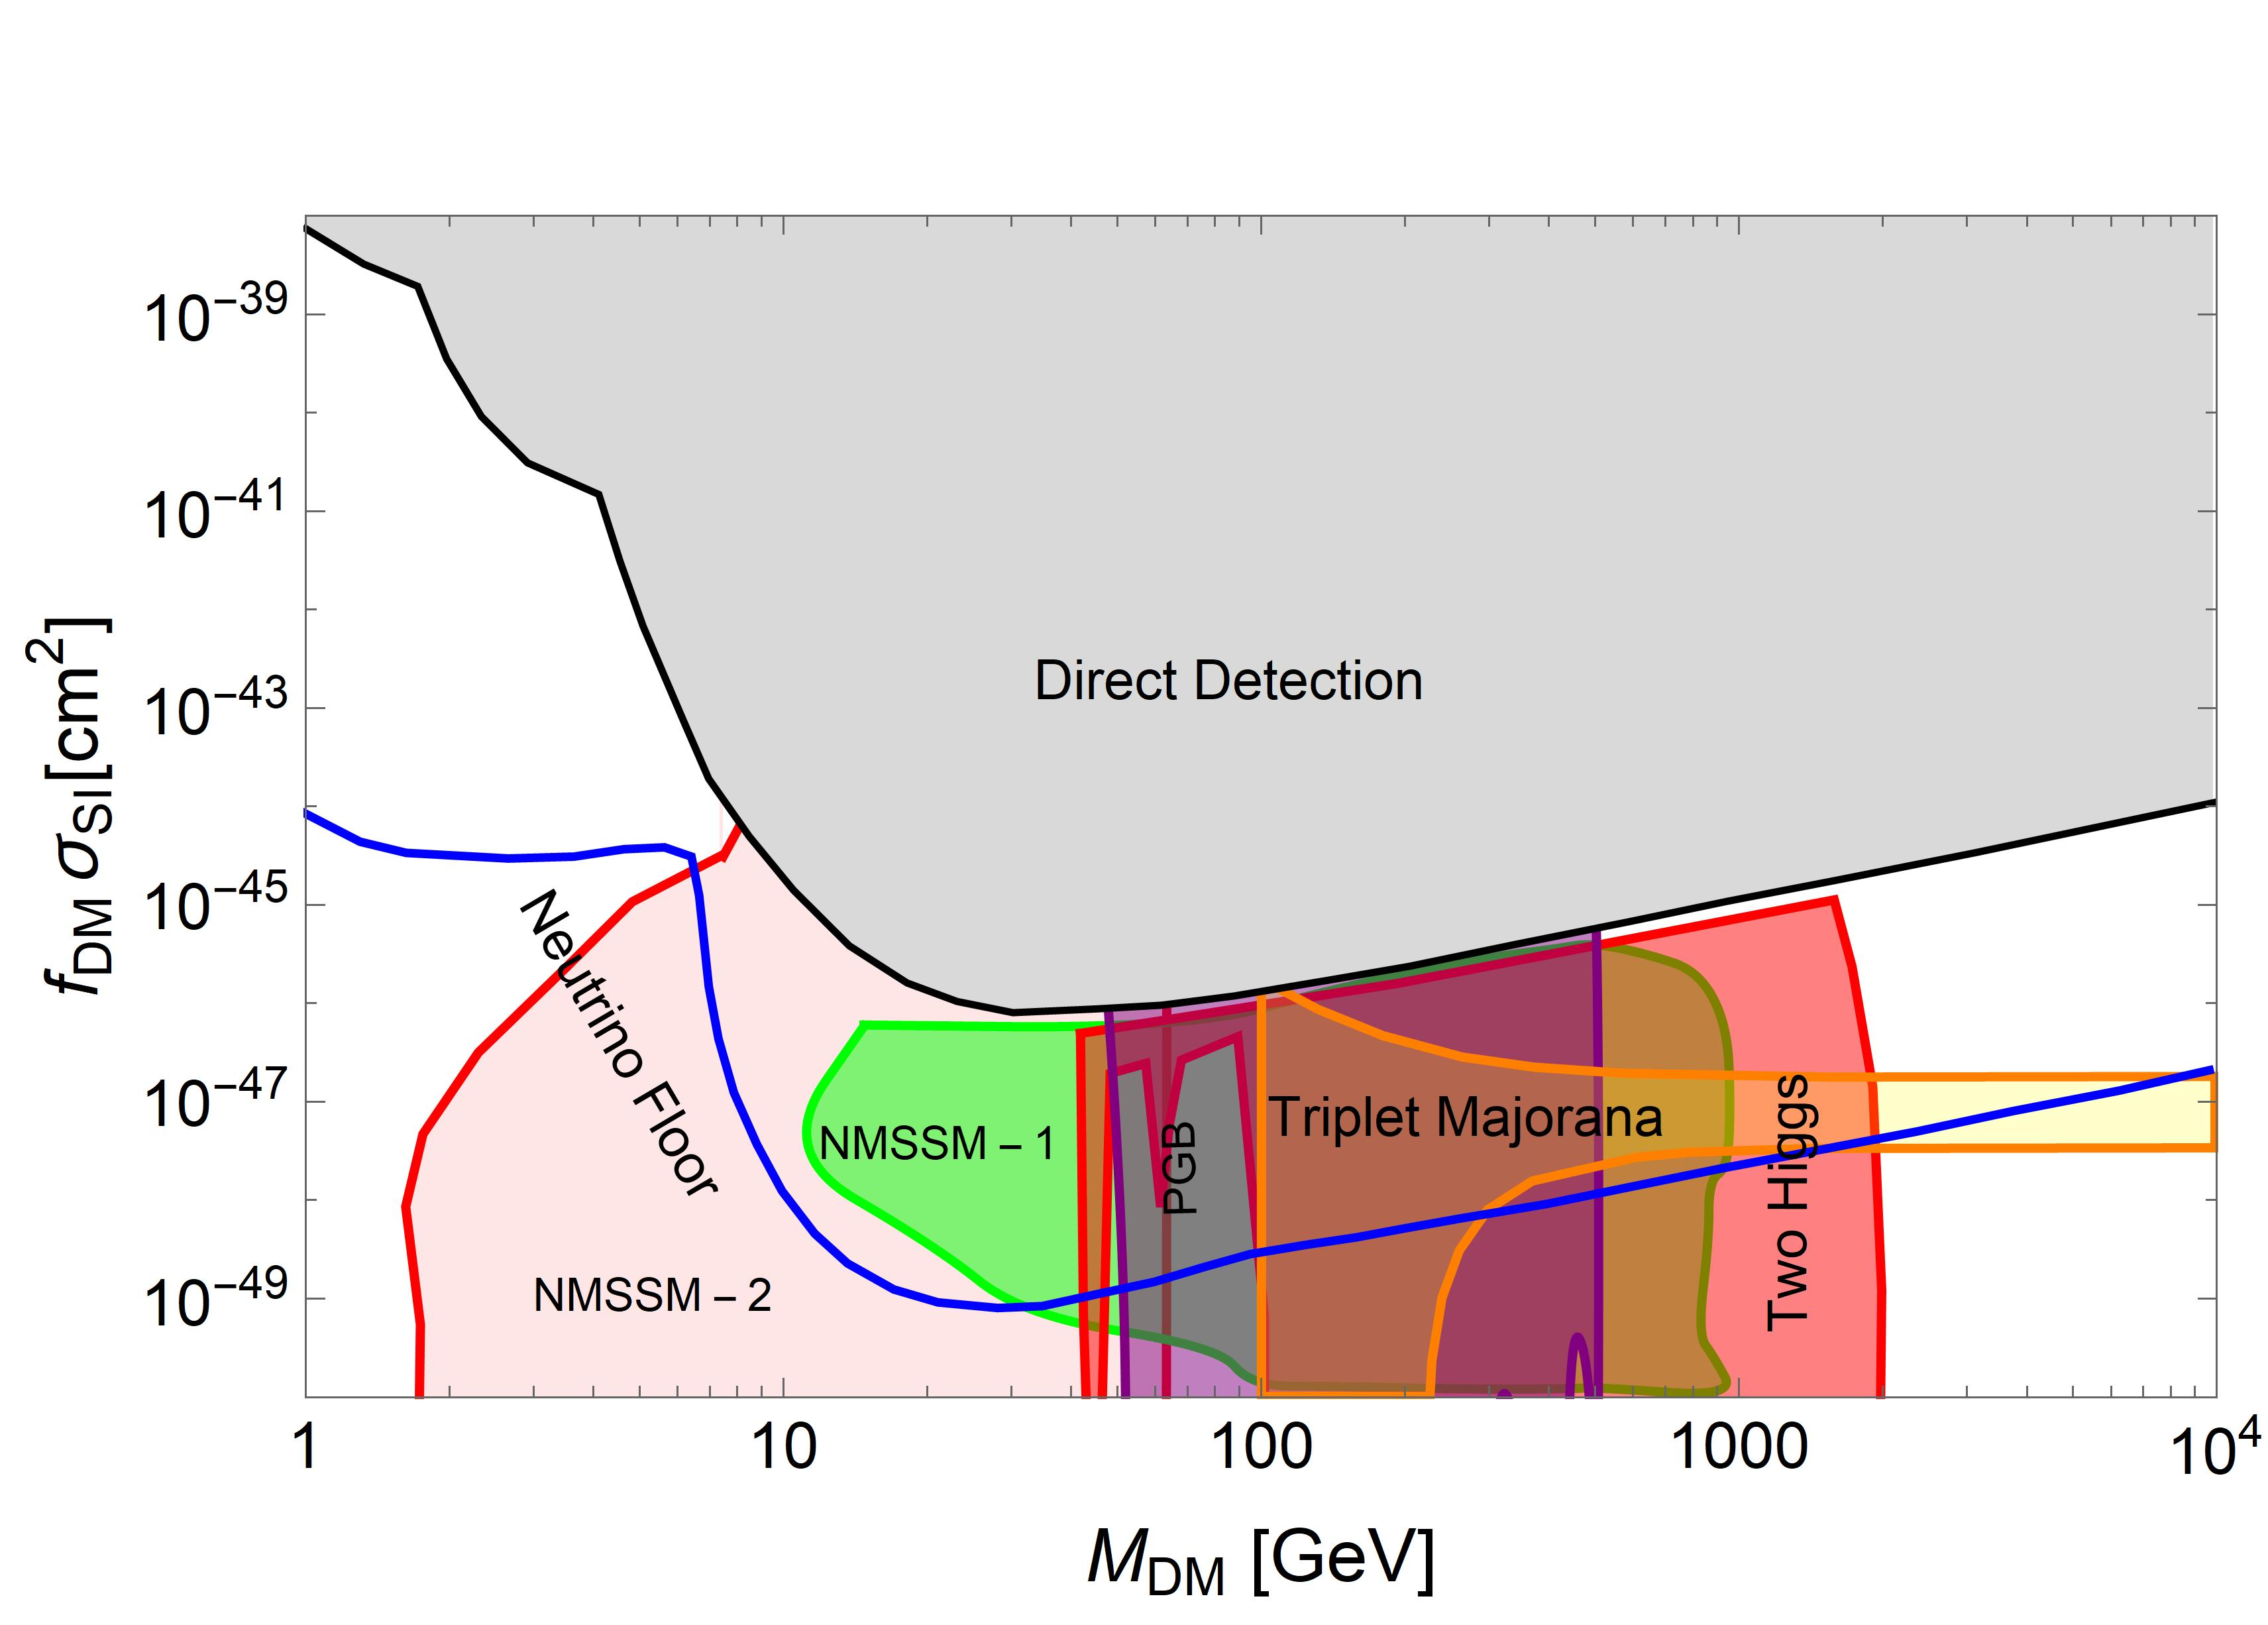
\includegraphics[width=0.65\columnwidth]{figures/sigmap_visible_plot.jpg}
\caption{Plots of dark matter-proton cross section $\sigma_{\rm SI}$  times dark matter fraction $f_{\rm DM}$ versus particle mass $M_{\rm DM}$ for SI scattering cross sections off nuclei. Examples of predicted regions in several visible sector models are reproduced: the NMSSM models of~\cite{Lopez-Fogliani:2021qpq} (``NMSSM-1", in green) and of \cite{Wang:2020xta} (``NMSSM-2", in pink), the two Higgs doublet model of~\cite{Cabrera:2019gaq} (``Two Higgs", in red), the pseudo-Goldstone boson  of~\cite{Alanne:2020jwx} (``PGB", in purple) and the electroweak triplet Majorana dark matter model of~\cite{Chen:2018uqz} (``Triplet Majorana", in yellow - however note that the relic abundance for this model was not computed). The gray region is excluded by existing direct detection limits~\cite{Evans:2017kti} and the blue line indicates the neutrino fog level in xenon~\cite{Billard:2013qya,Ruppin:2014bra}. Regions predicted by other examples of models mentioned in the text~\cite{VanBeekveld:2021tgn, Mukherjee:2022kff, Khater:2021wcx, Chen:2018uqz, Chen:2019gtm,Berlin:2015ymu} overlap with those shown and were not included for clarity.}
\label{fig:sample_SI-VisibleSector}
\end{center}
\end{figure}
 
 We classify dark matter models as either ``visible sector" or ``dark sector".
 Visible sector models include mostly particles that carry quantum numbers of the SM gauge group. They consist of extensions of the SM,  such as those supersymmetric or with multiple Higgs fields. By contrast, dark sector (or hidden sector) models contain many particles that do not interact with the SM, or interact only through a small mixing with it, often referred to as a ``portal".  The particles of the dark sector typically interact among themselves through new forces (Abelian or non-Abelian gauge groups) which could be spontaneously broken or confining.
 A dark sector could in principle be limited to gravitational interactions with the SM particles, but in this case there is no clear way to ensure that its relic density will appropriately match cosmological observations.  For this reason, the
 portal interactions of a dark sector model are typically essential to determine the dark matter abundance. Given the rich spectrum of the possible production mechanisms, the range of favored dark matter masses is typically wider in dark sector models than in visible sector ones. 
 
 In complete visible sector models, all scattering cross sections with the SM particles can be computed exactly, and cosmological and experimental limits applied to them. Some examples of this type are NMSSM models of~\cite{Lopez-Fogliani:2021qpq} and~\cite{Wang:2020xta}, the Phenomenological Minimal Supersymmetric Models (pMSSM) of~\cite{VanBeekveld:2021tgn} and~\cite{Mukherjee:2022kff}, the multiple scalar doublet models of~\cite{Cabrera:2019gaq} and ~\cite{Khater:2021wcx}, the $U(1)_{L\mu -L\tau}$ gauge SM extension model of~\cite{Singirala:2021gok}, the stable neutral heavy Dirac fermion dark matter (RHN model) in~\cite{Barger:2008qd}, 
 and the pseudo-Goldstone Boson dark matter model of \cite{Alanne:2020jwx}, in which the dark matter consists WIMPs of mass in the GeV to 1.5 TeV range with Spin Independent (SI) or Spin Dependent (SD)  scattering  cross sections off of nuclei.  
 In some visible sector models detailed predictions of the cross section of scattering of the dark matter off nuclei were made while remaining agnostic about how the dark matter relic density could be produced in the early Universe (e.g. for Higgsino like or Wino like fermions of 0.1 to 10 TeV mass in \cite{Chen:2018uqz} and \cite{Chen:2019gtm}). This approach can be motivated by our lack of knowledge of the cosmology during the epoch in which the DM relic abundance in these models is produced (see e.g.~\cite{Gelmini:2006pw, Gelmini:2006pq, Gelmini:2006mr, Berger:2020maa, Dienes:2021woi, Howard:2021ohe}).  In this case, one should be aware that different assumptions about the dark matter production would typically select only a small portion of the parameter space considered.
 
 In Fig.~\ref{fig:sample_SI-VisibleSector} we reproduce some of the predictions for SI scattering cross sections (in plots of dark matter-proton cross section versus dark matter mass)  for the visible sector models of Refs.~\cite{Lopez-Fogliani:2021qpq, Wang:2020xta, Cabrera:2019gaq, Alanne:2020jwx, Chen:2018uqz}. Examples of predictions of dark sector model models for SI scattering  are shown in Fig.~\ref{fig:sample_SI-DarkSector}, as explained below. 

In Fig.~\ref{fig:sample_SD-VisibleSector} we reproduce some of the predictions for SD scattering cross sections (in plots of dark matter-proton cross section versus dark matter mass)  for the visible sector models of Refs.~\cite{Lopez-Fogliani:2021qpq, Wang:2020xta, VanBeekveld:2021tgn, Singirala:2021gok, Barger:2008qd}. 

 
\begin{figure}[h]
\begin{center}
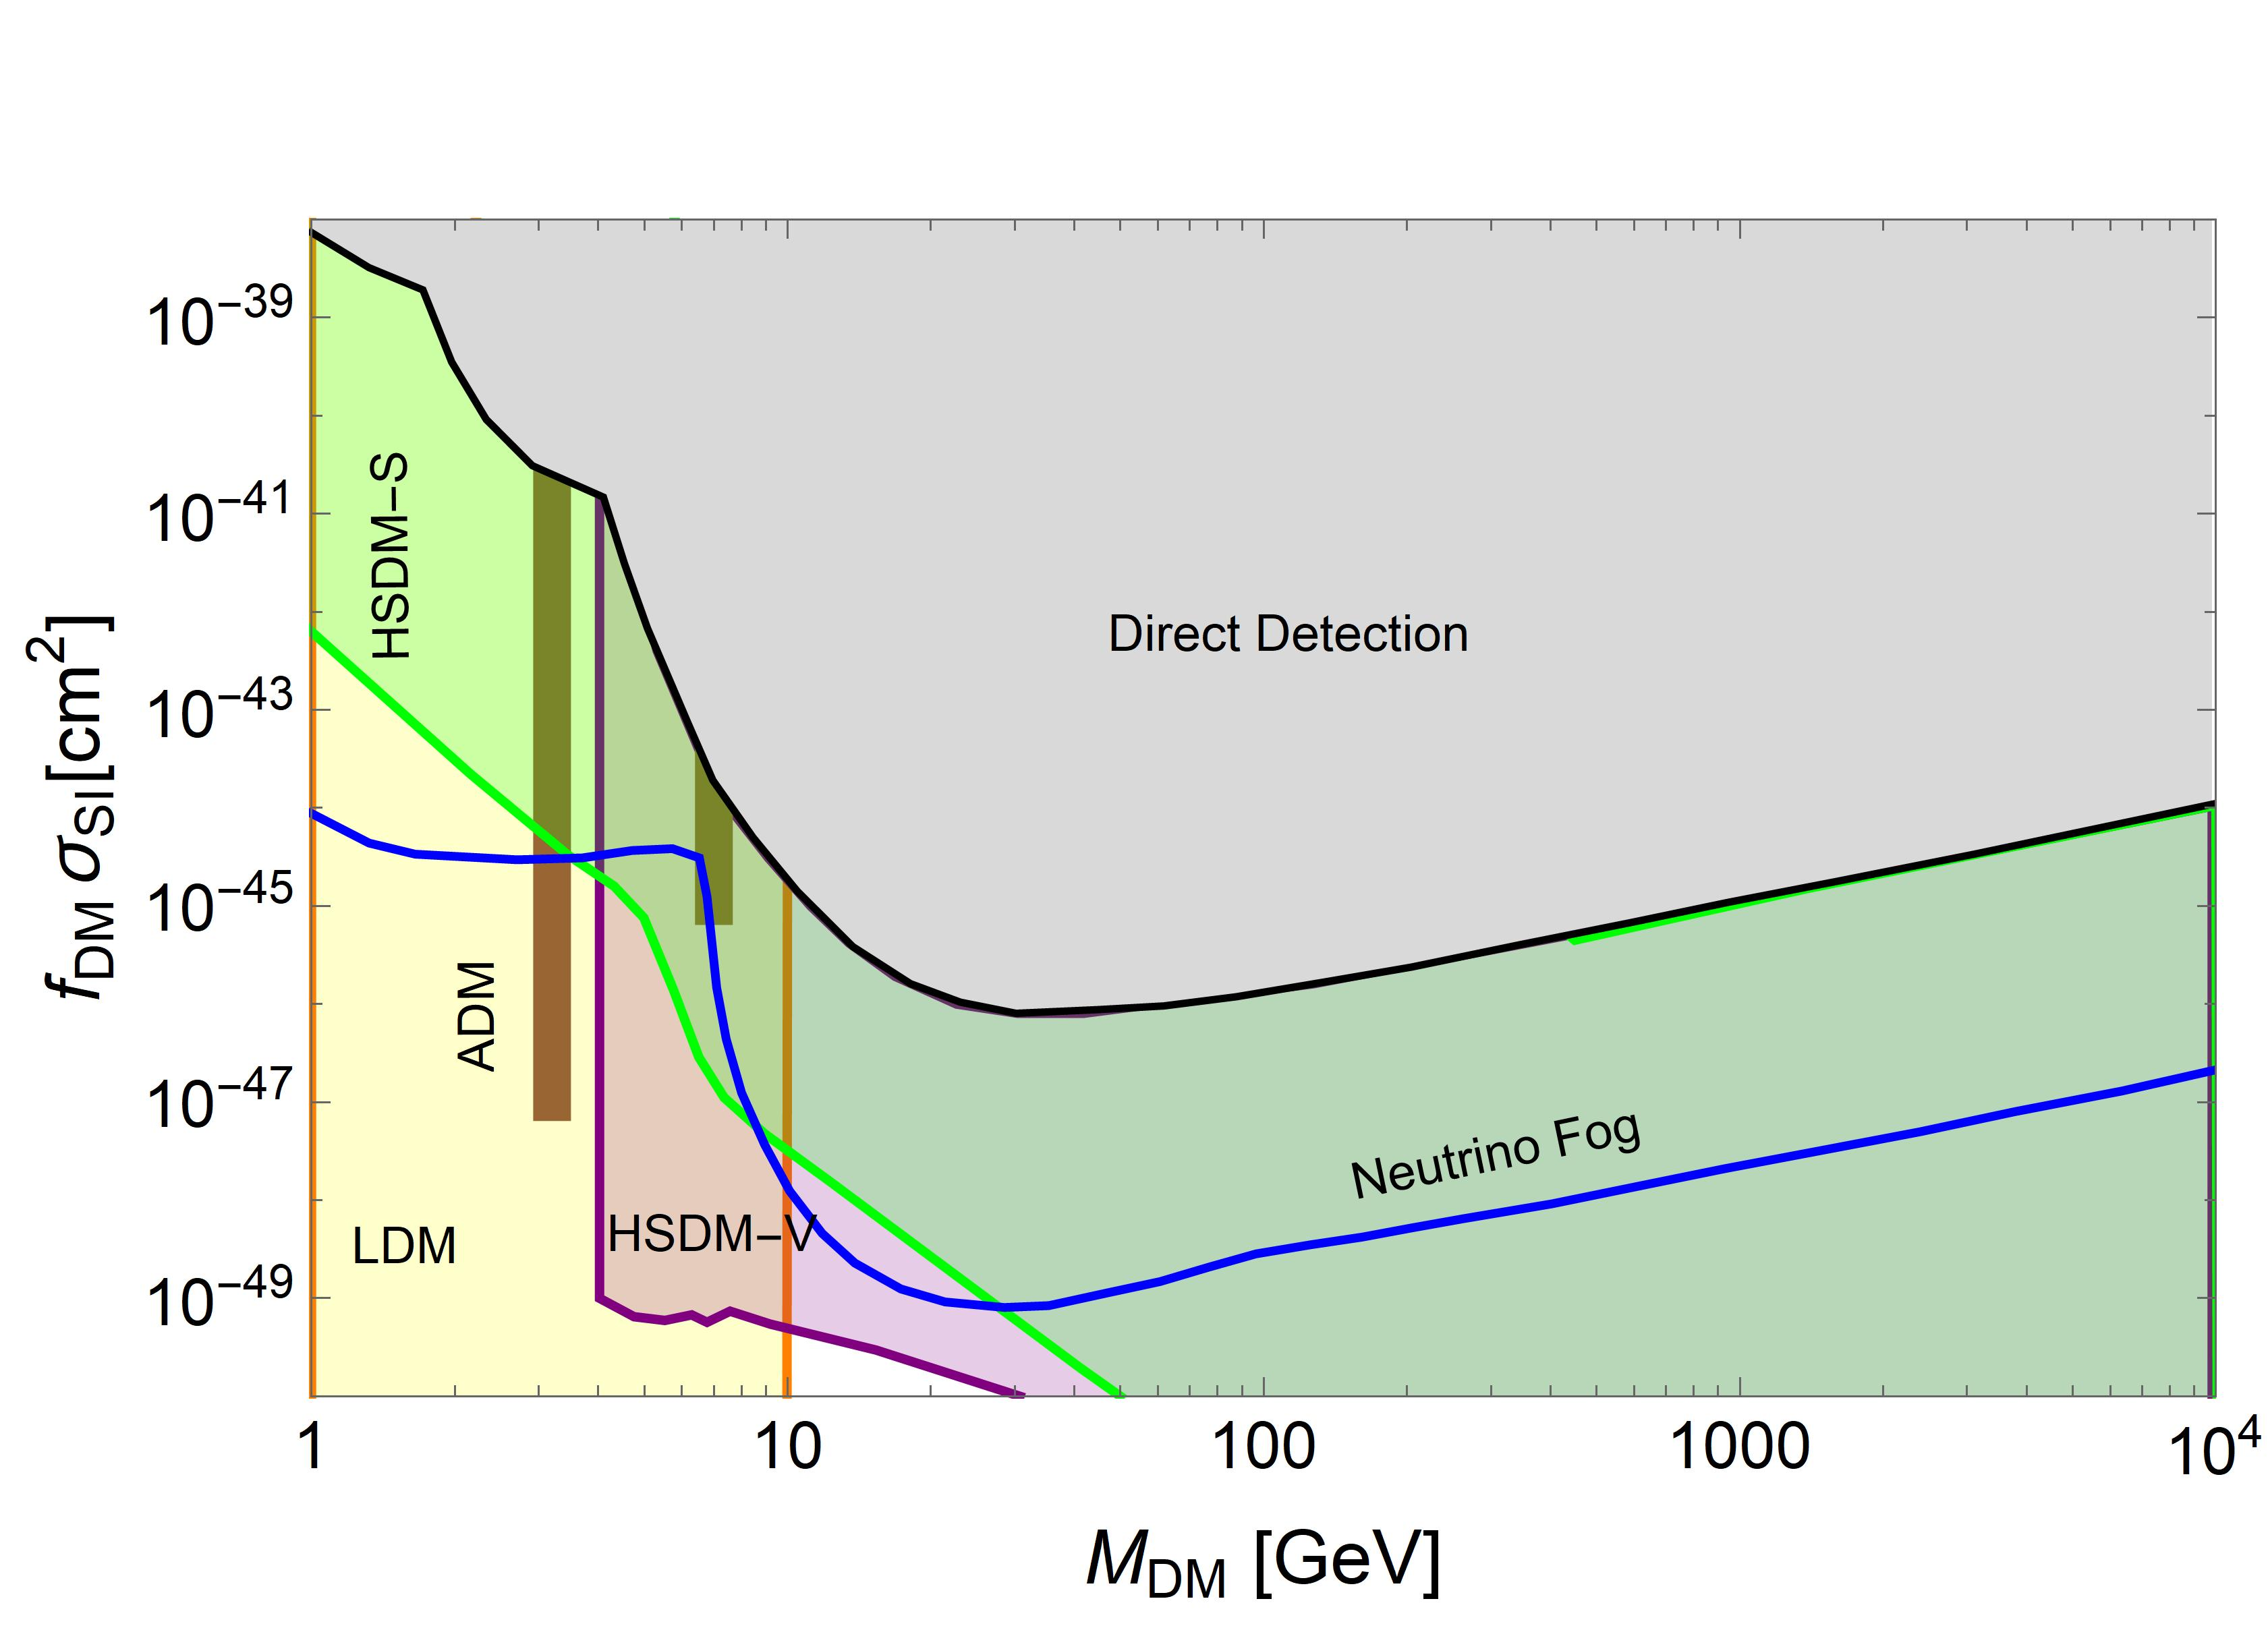
\includegraphics[width=0.65\columnwidth]{figures/sigmap_plot.jpg}
\caption{Same as in Fig.~\ref{fig:sample_SI-VisibleSector} for SI cross sections but for a few dark sector models: the minimal hidden sector dark matter models of~\cite{Evans:2017kti} with a vector portal (``HSDM-V", in purple) and with a Higgs scalar portal (``HSDM-S", in green), the asymmetric dark matter model of~\cite{Cohen:2010kn} (``ADM", brown vertical bars) and the symmetric and asymmetric light dark matter models of~\cite{Lin:2011gj} (``LDM", in yellow).}
\label{fig:sample_SI-DarkSector}
\end{center}
\end{figure}

\begin{figure}[t]
\begin{center}
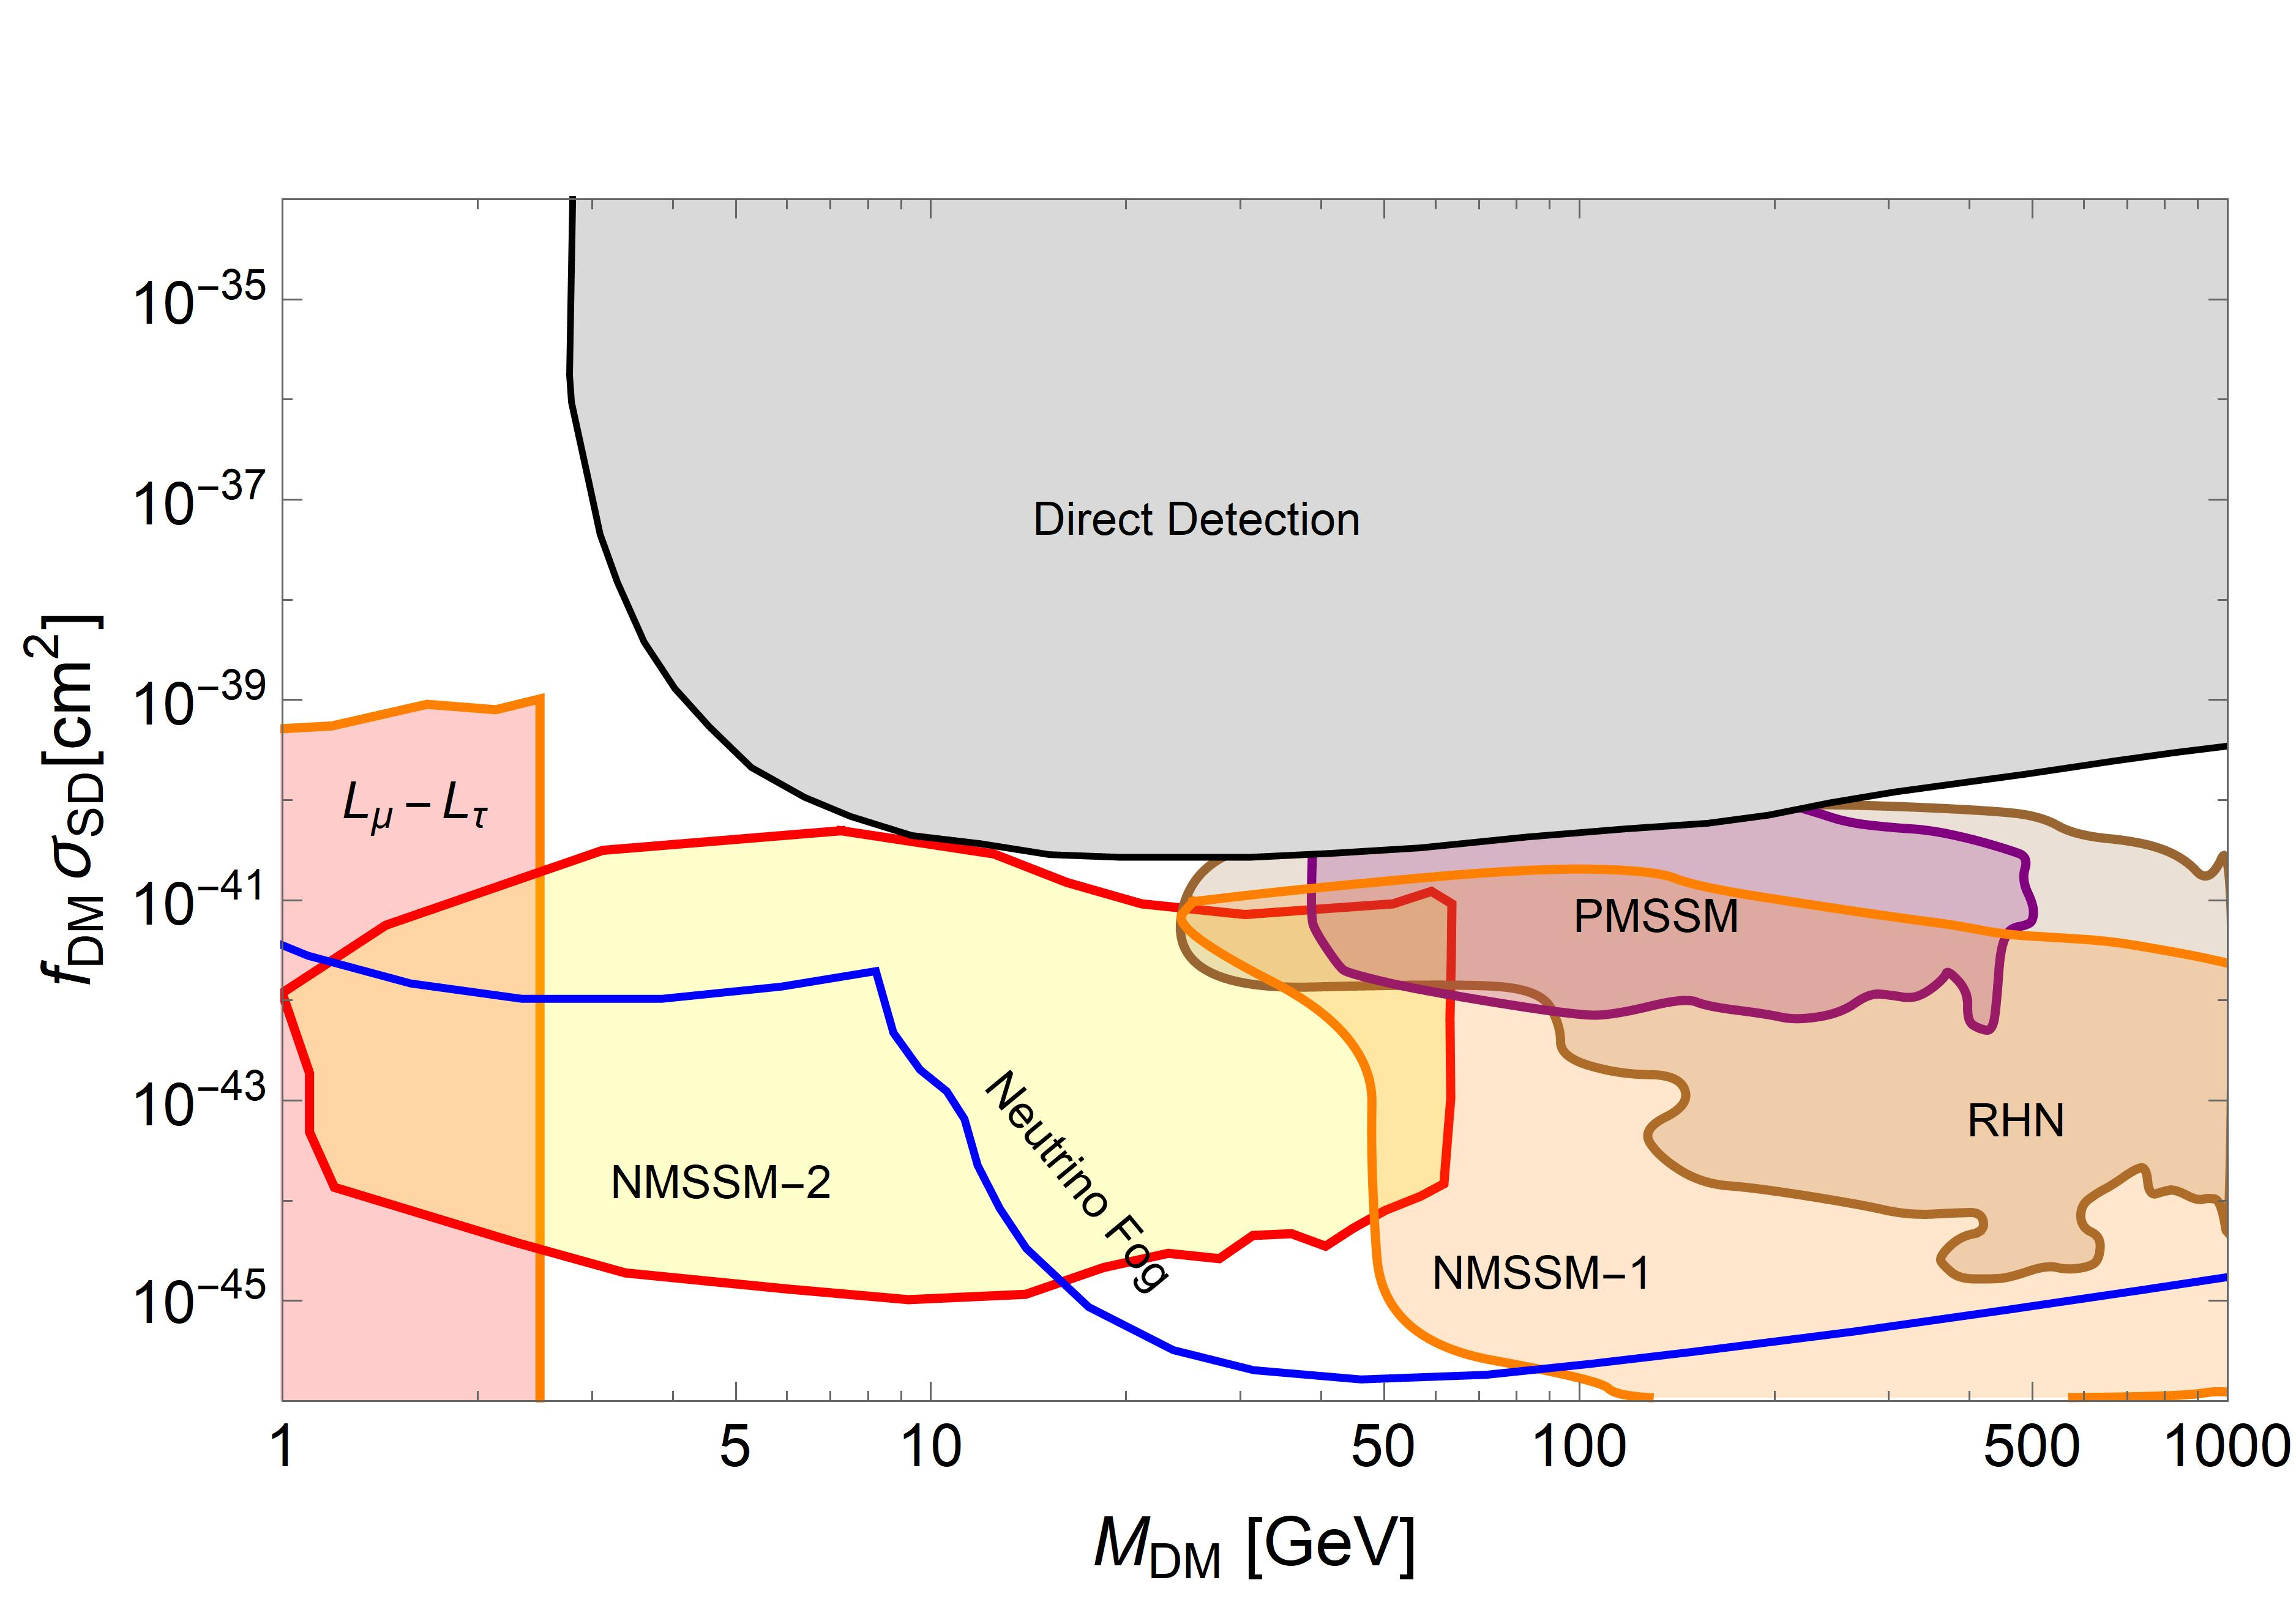
\includegraphics[width=0.65\columnwidth]{figures/sigmapSD_plot.jpg}
\caption{Plots of dark matter-proton cross section $\sigma_{\rm SD}$  times dark matter fraction $f_{\rm DM}$ versus particle mass $M_{\rm DM}$ for SD scattering cross sections off nuclei. Examples of predicted regions in several visible sector models are reproduced: the NMSSM models of~\cite{Lopez-Fogliani:2021qpq} (``NMSSM-1", in orange) and of \cite{Wang:2020xta} (``NMSSM-2", in yellow), the pMSSM model of~\cite{VanBeekveld:2021tgn} (``pMSSM", in purple), the $U(1)_{L\mu -L\tau}$ gauge SM extension model of~\cite{Singirala:2021gok} (``$L_\mu - L_\tau$", in pink), the heavy Dirac fermion model in~\cite{Barger:2008qd} (``RHN", in brown). The gray region is excluded by existing direct detection limits and the blue line indicates the neutrino fog level in for C$_3$F$_8$~\cite{Ruppin:2014bra}.}
\label{fig:sample_SD-VisibleSector}
\end{center}
\end{figure}

 Complete dark sector models exist in which the dark matter interaction with the visible sector is required as an integral ingredient to successfully predict the dark matter abundance. One of the most predictive is the ``Elastically Decoupling Relic" (ELDER) dark matter model \cite{Kuflik:2015isi, Kuflik:2017iqs}, a thermal relic whose present density is determined primarily by the cross-section of its elastic scattering off SM particles. Assuming this scattering is mediated by a kinetically mixed dark photon, the ELDER model makes concrete predictions for scattering off electrons. In this model the dark matter has strong number-changing self-interactions.  This is also the case for the “Strongly-Interacting Massive Particle” (SIMP) model of~\cite{Hochberg:2014dra}, where the relic abundance is determined by the strong self interactions, with the coupling to the visible sector necessary to maintain thermal equilibrium between the SM and dark sector. Without thermal equilibrium, 3 to 2 annihilation would heat up the DM through ``cannibalization"~\cite{Boddy:2014yra, Carlson:1992fn}, resulting in large velocities incompatible with observations of structure formation in the Universe. ELDER and SIMP model predictions are shown in Fig.~\ref{fig:sample_electron}.
 
\begin{figure}[t]
\begin{center}
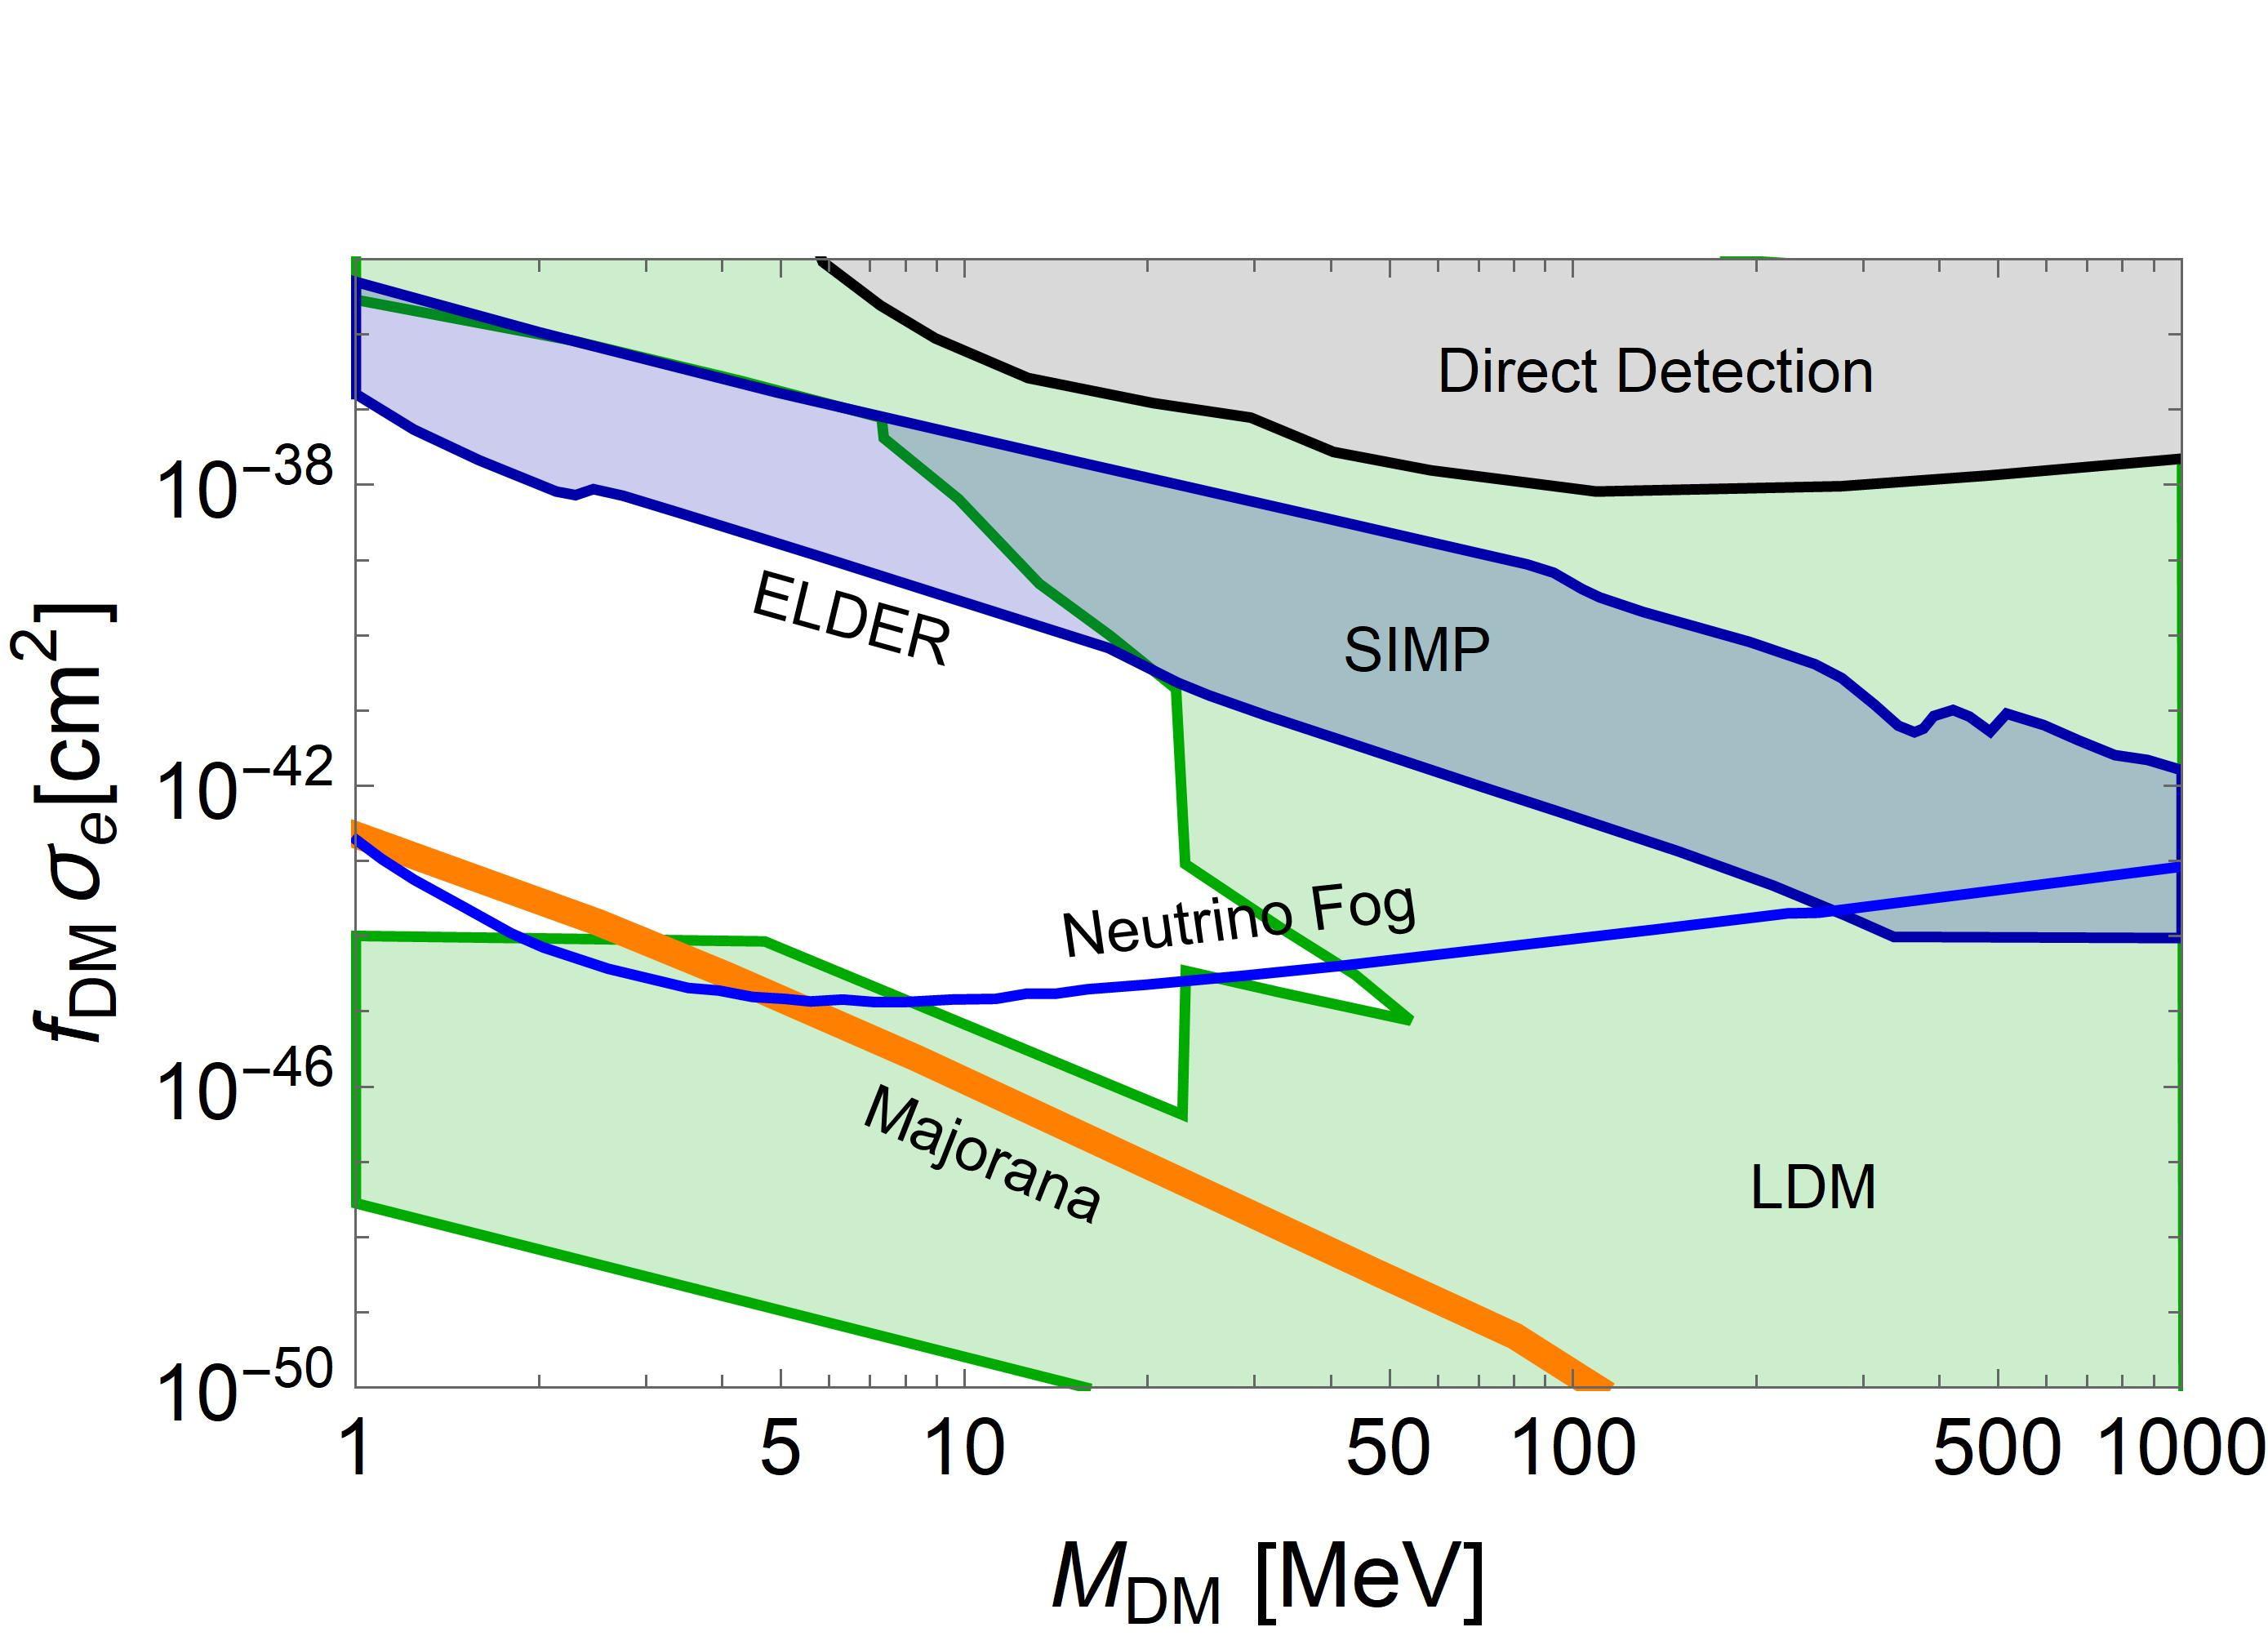
\includegraphics[width=0.65\columnwidth]{figures/sigmae_plot.jpg}
\caption{Dark matter-electron scattering cross section $\sigma_e$ times dark matter fraction $f_{\rm DM}$ versus particle mass $M_{\rm DM}$. Examples of predicted regions in several models are reproduced: the
$f_{\rm DM}=1$ line for the ELDER model and region for the SIMP model of~\cite{Kuflik:2017iqs} (in blue), the Majorana dark matter line of Fig 6 of~\cite{Battaglieri:2017aum} (in orange), the symmetric and asymmetric light dark matter (LDM) region of~\cite{Lin:2011gj} (in green). The 100\% discrimination $F_{\rm DM } = 1$ neutrino fog level for a $10^5$ kg-y exposure of~\cite{Wyenberg:2018eyv}(blue line) and the region rejected by present direct detection constraints (in gray) are shown for comparison.}
\label{fig:sample_electron}
\end{center}
\end{figure}

 
Simplified models are defined by a small number of new particles and their interactions, often restricted to a single interaction channel with the SM that is assumed to dominate, while remaining agnostic about others that would be likely to appear in a more complete model.  Some simplified models take into account all cosmological, astrophysical and experimental bounds that apply to them, e.g. those mentioned in this paragraph. 
In the asymmetric dark matter (ADM) from a GeV hidden sector model of~\cite{Cohen:2010kn}, the scattering off nuclei is computed for a few illustrative dark matter  masses -- for a mass of 3.3 GeV, the scattering cross section is close to the neutrino fog (as shown in Fig.~\ref{fig:sample_SI-DarkSector}). 
 In the symmetric and asymmetric dark matter dark sector models of~\cite{Lin:2011gj}, a dark matter particle of mass in the 1 MeV to 10 GeV range could scatter off nuclei (covering all the allowed region shown in Fig.~\ref{fig:sample_SI-DarkSector}) or electrons (as shown in Fig.~\ref{fig:sample_electron})  with cross sections close to the respective neutrino fog levels. 
 In the minimal hidden sector dark models of~\cite{Evans:2017kti}, dark matter with SI scattering off nuclei at the neutrino fog level can have masses in the 0.5 GeV to 10 TeV range (see Fig.~\ref{fig:sample_SI-DarkSector})
In the visible sector Majorana fermion dark matter models of~\cite{Berlin:2015ymu}, SI scattering off of nuclei is predicted at loop level to lie at or just below the neutrino fog for dark matter masses from 0.1 to 1 TeV. 
In~\cite{Battaglieri:2017aum}  a specific example of a Majorana fermion scattering off electrons is given whose cross section  would encounter the neutrino fog (the corresponding line in Fig.~6 of~\cite{Battaglieri:2017aum} is reproduced in Fig.~\ref{fig:sample_electron}).

 
 
  Fig.~\ref{fig:sample_electron}  shows the ELDER line and SIMP region predicted in~\cite{Kuflik:2017iqs} for scattering off electrons of 1 MeV to 1 GeV dark matter particles and the region of models of~\cite{Lin:2011gj}, the symmetric and asymmetric light dark matter (LDM) region of~\cite{Lin:2011gj} and the Majorana dark matter line of Fig 6 of~\cite{Battaglieri:2017aum} (in orange),   The 100\% discrimination $F_{\rm DM } = 1$ neutrino floor level for a $10^5$ kg-y exposure of~\cite{Wyenberg:2018eyv} is shown in the figure for comparison (higher fog levels for scattering off electrons corresponding to smaller exposures where computed in~\cite{Essig:2018tss}).

 
 Dark matter particles could also interact with SM particles through electromagnetic multipole moments, leading to scattering with a very different momentum transfer dependence from the usual SI or SD cases.   Many models realize this idea for fermionic or vectorial dark matter. E.g. the particular vectorial DM model of~\cite{Hisano:2020qkq} shows predictions for scattering cross sections which extend to and into the neutrino fog.  However, one should bear in mind that the relic dark matter abundance and cosmological bounds were not computed.  
 
Finally, we mention two approaches to modeling DM interactions which are completely agnostic with regard to the size of the scattering cross section. 
In the first, a single interaction channel between the DM and the SM mediated by a single messenger is considered (see e.g.~\cite{Gelmini:2018ogy}).  Typically such simplified models consist of Lagrangian terms defining the messenger couplings to the DM and to quarks and/or electrons and a type and mass of the single mediator. The simplest incarnations thus are defined by four parameters: the two coupling constants, the DM mass, and the mediator mass,
with the advantage that the spectrum and experimental signals are relatively easy to understand.  The disadvantage is that in more realistic models, there are often several relevant messengers and/or interactions, whose relative importance often varies across the parameter space and for the various experimental searches (see e.g.~\cite{Profumo:2013hqa}).

A second approach is that of studying single non-relativistic effective field theory (NR EFT) of dark matter-nucleus coupling, a theoretical framework describing different types of nuclear response to dark matter scattering which yields insight into different viable dark matter couplings~\cite{Fitzpatrick:2012ix}. However, most of the dark matter-nuclei interactions defined in terms of a field theoretical Lagrangian formalism involve complex linear combinations of EFT operators in the non-relativistic limit, with the relative importance of each EFT operator weighted by nuclide-specific factors, and realistic relativistic constructions typically require several NR EFT operators for an accurate description (see e.g.~\cite{Gresham:2014vja}).

The examples we provide show that a large variety of dark matter models predict scattering cross sections at or below the neutrino fog.

